\begin{document}

	\frame{\titlepage}

	\section{Architectural Highlights}

	\begin{frame}
		\frametitle{Machine Type}

		\begin{itemize}
			\item Machine Type
				\begin{itemize}
					\item 8 registers
						\begin{itemize}
							\item No special registers
							\item Hardwired role in branching, accessing data memory, and the ALU
						\end{itemize}
					\item Accumulator
						\begin{itemize}
							\item Hardwired role in branching, accessing data memory, and the ALU
						\end{itemize}
					\item Load-Store
						\begin{itemize}
							\item Data must be loaded to the accumulator or a register before being used
							\item Instructions to load/store to/from data memory
						\end{itemize}
				\end{itemize}
			\item Number of registers: 8 registers + accumulator
		\end{itemize}
	\end{frame}
	\begin{frame}
		\frametitle{Instruction Format}

		\begin{itemize}
			\item Instruction format:

				\begin{table}
					\begin{tabular}{|c|c|c|c|c|c|c|c|c|}
						\hline
						8 & 7 & 6 & 5 & 4 & 3 & 2 & 1 & 0 \\ \hline
						\multicolumn{5}{|c|}{Opcode} & i & \multicolumn{3}{|c|}{val} \\ \hline
					\end{tabular}
				\end{table}

				\begin{itemize}
					\item[Opcode:] The opcode
					\item[i:] Toggles registers vs immediates; 0 for registers, 1 for immediates
					\item[val:] The register number or the immediate
				\end{itemize}

				\begin{itemize}
					\item Not all instructions require \texttt{i} and/or \texttt{val}
				\end{itemize}
		\end{itemize}
	\end{frame}

	\begin{frame}[fragile]
		\frametitle{Instructions}

		\begin{itemize}
			\small
			\item[A:] Value in the accumulator
			\item[val:] The value referenced by the \texttt{val} and \texttt{i} fields of the instruction \\
		\end{itemize}

		\begin{table}[]
			\tiny
			\begin{tabular}{|c|c|l|}
				\hline
				Instruction & Op & Explanation \\ \hline
				add & 0 & \texttt{A += val} \\
				sub & 1 & \texttt{A -= val} \\ \hline
				and & 2 & \texttt{A \&= val} \\
				or & 3 & \texttt{A |= val} \\
				xor & 4 & \verb|A ^= val| \\ \hline
				dand & 5 & \verb|A = &(A[7:0], val[7:0])| \\
				dor & 6 & \verb/A = |(A[7:0], val[7:0]) / \\
				dxor & 7 & \verb|A = ^(A[7:0], val[7:0])| \\ \hline
				sl & 8 & \verb|A <<= val| \\
				sr & 9 & \verb|A >>= val| \\ \hline
				emsw & 10 & \multirow{2}{25em}{Extract the output MSW/LSW for encoding} \\
				elsw & 11 & \\
				dmsw & 12 & \multirow{2}{25em}{Extract the MSW/LSW for decoding} \\
				dlsw & 13 & \\ \hline
				xp4 & 14 & \multirow{3}{25em}{Puts the relevant bits in the accumulator, including the parity bit. MSW should be in $A$ and LSW should be in $val$.} \\
				xp2 & 15 & \\
				xp1 & 16 & \\ \hline
				loadm & 17 & $A \leftarrow \op{Mem}[val]$ \\
				loadv & 18 & $A \leftarrow val$ \\
				storem & 19 & $\op{Mem}[val] \leftarrow A$ \\
				storev & 20 & $val \leftarrow A$. Writes register; behavior when \verb|i == 0| is undefined \\ \hline
				slt & 21 & \\
				beq & 22 & \\
				rb & 23 & \\
				ab & 24 & \\ \hline
				done & 31 & Sets the \verb|done| flag to indicate the program has finished \\
				\hline
			\end{tabular}
		\end{table}
	\end{frame}

	%\section{Block Diagram}

	\begin{frame}
		\frametitle{Data Path Diagram}

		\begin{figure}[h]
			\includegraphics[height=7cm]{data-path-diagram}
			\caption{Data path Diagram (No control signals)}
		\end{figure}
	\end{frame}

	\begin{frame}
		\frametitle{Block Diagram}
		\begin{figure}[h]
			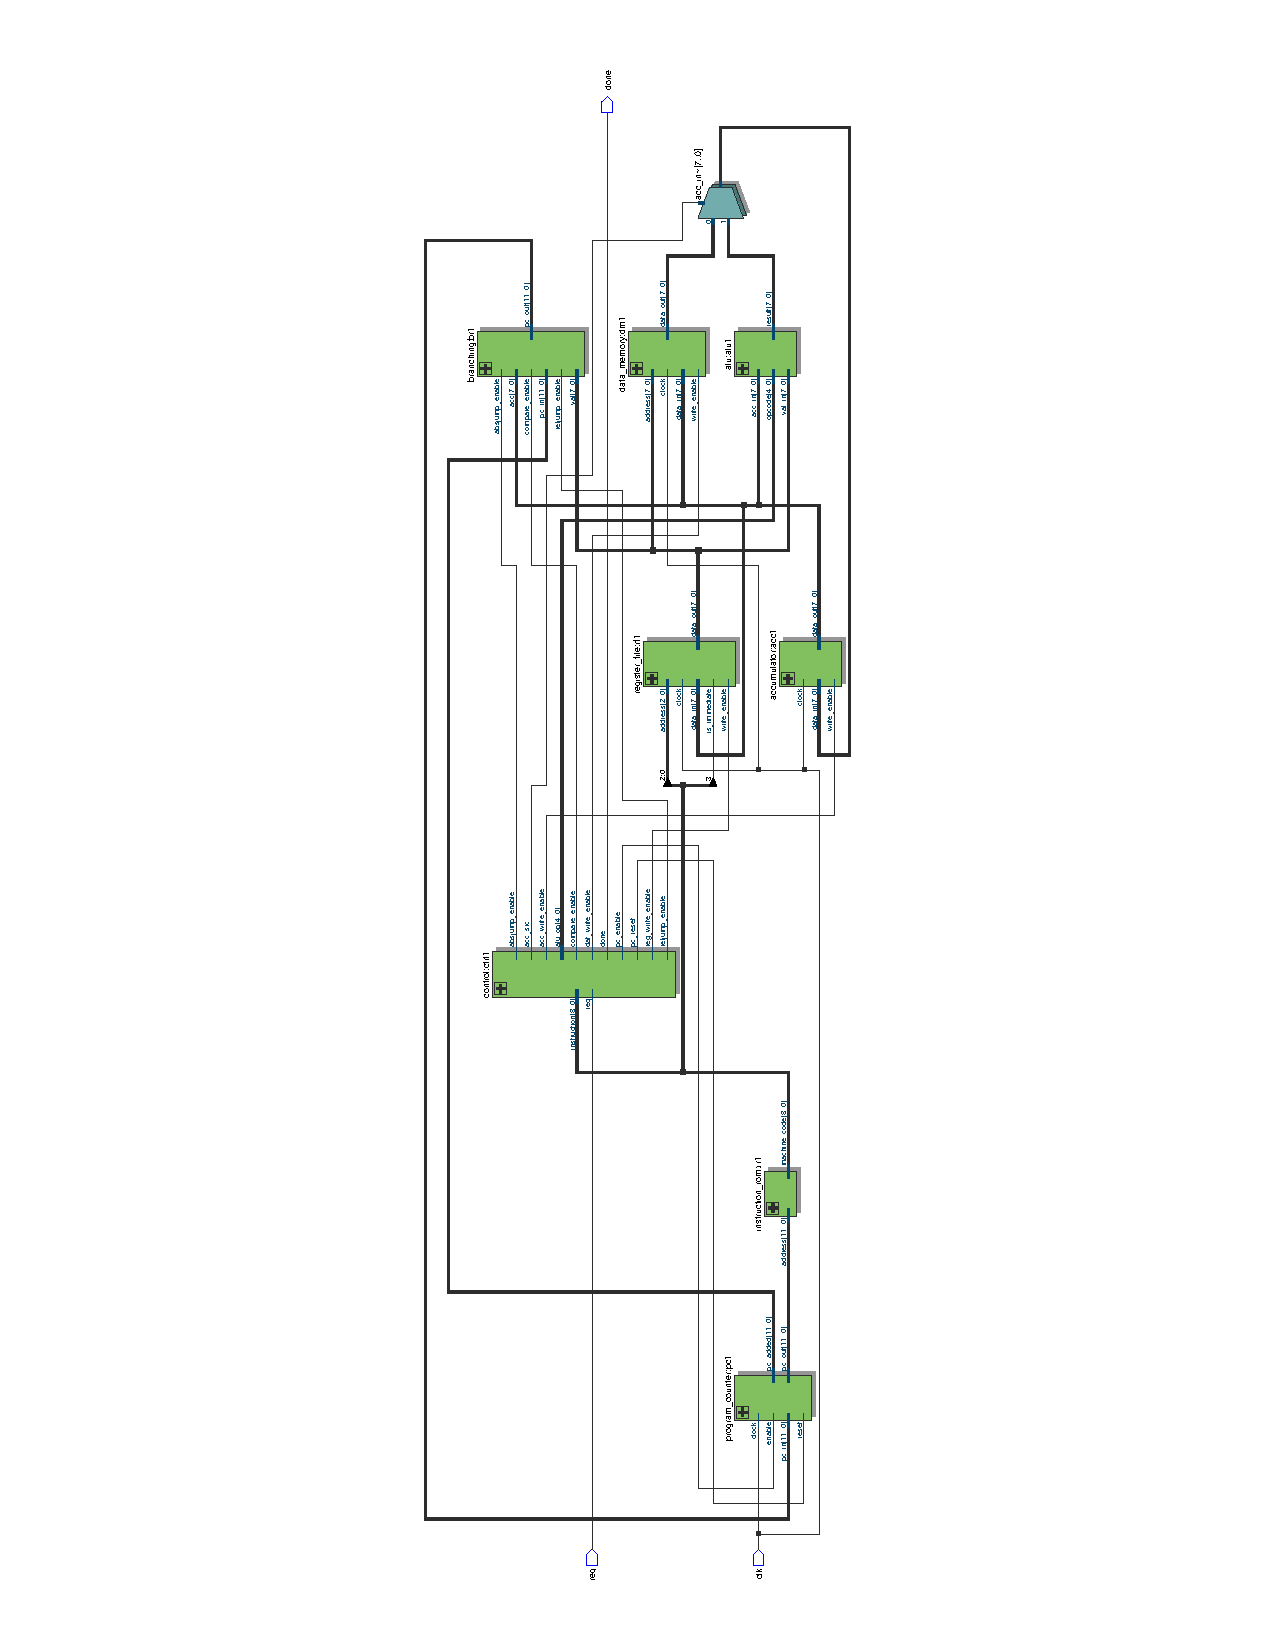
\includegraphics[angle=270, trim={7cm 1.5cm 7cm 1.5cm}, width=\textwidth]{block-diagram}
			\caption{Full block diagram with control signals}
		\end{figure}
	\end{frame}

	\section{Explain Assembly}

	\begin{frame}
		\frametitle{Assembly Syntax}

		\begin{itemize}
			\item Example instruction:
				\begin{quote}
					\texttt{add~~~~~i 1}
				\end{quote}
			\item Amount of whitespace is ignored
			\item Leading/trailing whitespace is ignored
			\item Any text starting from a \texttt{\#} are comments is ignored
			\item Lines without an instruction are ignored
		\end{itemize}

	\end{frame}

	\begin{frame}
		\frametitle{Explain assembly: Data}

		\begin{itemize}
			\item Obtain Data
				\begin{itemize}
					\item Small constants (0-7) can be loaded as immediates (\texttt{load i 7})
					\item Larger constants must be assembled from smaller immediates using various instructions such as bit shifting and \texttt{or}.

						Example for loading $30$:
						\begin{quote}
							\normalfont{\texttt{loadv~~~i 7 \\
							sl~~~~~~i 3 \\
							or~~~~~~i 2 \\
							}}
						\end{quote}
				\end{itemize}
			\item Manipulate Data
				\begin{itemize}
					\item Put one operand in accumulator
					\item Put other operand in register or use immediate
					\item Result is in the accumulator
				\end{itemize}
			\item Store results
				\begin{itemize}
					\item To registers: \texttt{storev}
					\item To data memory: \texttt{storem}
						\begin{itemize}
							\item[Note:] Data will not be available from register for the next instruction, so a NOP or other instruction between is necessary. Don't rely on this either because the only reason for this behavior is to not change the hardware when not necessary
						\end{itemize}
				\end{itemize}
		\end{itemize}
	\end{frame}

	\begin{frame}
		\frametitle{Explain Assembly: Subroutines/Jumps}

		\begin{itemize}
			\item Conditional jumps
				\begin{itemize}
					\item \texttt{beq}: If \texttt{A == 0} then branch forward by \texttt{val} instructions
				\end{itemize}
			\item Unconditional jumps
				\begin{itemize}
					\item \texttt{rb}: Branch forward by \texttt{val} instructions
					\item {ab} Branch to the \texttt{(val << 2)}th instruction. Use NOP padding if necessary.
				\end{itemize}
			\item Other:
				\begin{itemize}
					\item Backward conditional jump: Use \texttt{beq} to branch over instructions that absolute branch to the jump location
					\item Branch over branch instructions
					\item Load larger constants to a register to branch larger distances or to larger absolute addresses
				\end{itemize}
		\end{itemize}
	\end{frame}

	\begin{frame}
		\frametitle{Explain Assembly: Program 1}
		\begin{itemize}
			\item Loop through all messages
				\begin{itemize}
					\item Load input data
					\item Set data bits in output data (in registers)
					\item Extract and set parity bits
					\item Store output data
				\end{itemize}
			\item done
		\end{itemize}
	\end{frame}

	\begin{frame}
		\frametitle{Explain Assembly: Program 2}
		\begin{itemize}
			\item Let $S_8, S_4, S_2, S_1, S_2$ be parity calculated from input
			\item for each message
				\begin{itemize}
					\item Read message from data memory
					\item Create $p=\{S_8, S_4, S_2, S_1\}$
					\item If $S_0 = 0$: 0 or 2 errors
						\begin{itemize}
							\item Extract and store LSW
							\item Extract MSW
							\item If $p = 0$: No errors: do nothing
							\item Else ($p \neq  0$): 2 errors: set bit
							\item Store MSW
						\end{itemize}
					\item Else: ($S_0 \neq 0$: 1 error)
						\begin{itemize}
							\item Flip $p^{th}$ bit in input message
							\item Extract data bits to output
							\item Set $F_0$
							\item Store output
						\end{itemize}
				\end{itemize}
			\item done
		\end{itemize}
	\end{frame}

	\begin{frame}
		\frametitle{Explain Assembly: Program 3}
		\begin{itemize}
			\item Load first byte
			\item Loop
				\begin{itemize}
					\item Count matches within current byte (loop)
					\item Update counters in memory for occurences with byte and bytes with pattern
					\item If no next byte: Update counter in memory and \texttt{done}
					\item Else
						\begin{itemize}
							\item Load next byte
							\item Count occurences in byte boundary
							\item Update counter in memory
							\item Reset counter
							\item current $\leftarrow$ next
						\end{itemize}
				\end{itemize}
			\item done
		\end{itemize}
	\end{frame}

	\section{Explain Testbench}

	\begin{frame}
		\frametitle{Explain Testbench}

		Using the provided test benches for each program.

		\begin{itemize}
			\item Load instruction memory from file
			\item Randomize input data
			\item Compute expected output
			\item Set data memory to input
			\item Run program until \texttt{done} flag
			\item Compare output from data memory to computed
		\end{itemize}
	\end{frame}

	\begin{frame}
		\frametitle{Testbench Results}

		\begin{itemize}
			\item Run each test bench in Questa to show
		\end{itemize}
	\end{frame}

	\section{Evaluate Performance}

	\begin{frame}
		\frametitle{Evaluate Performance}

		\begin{itemize}
			\item Accumulator machine + load-store means more instructions
			\item Higher instruction count for most things
				\begin{itemize}
					\item Using larger constants require multiple instructions
					\item Storing data after manipulating it requires a separate instruction
				\end{itemize}
			\item Some annoying bit-moving operations handled by a few specialized instructions, much less than otherwise.
		\end{itemize}
	\end{frame}

\end{document}
